\documentclass{article}
\usepackage[utf8]{inputenc}
\usepackage{amsmath}
\usepackage{graphicx}
\usepackage{minted}
\usepackage{subfigure}
\setminted{fontsize=\scriptsize,baselinestretch=1}

\title{Shared Memory Code Generation with Thorin}
\author{Rafael Ravedutti Lucio Machado }
\date{November 2017}

\begin{document}

\maketitle

\clearpage

\tableofcontents

\clearpage

\section{Introduction}
AnyDSL \cite{anydsl} is a framework designed for the development of domain specific libraries, it allows developers to split their work in application developer, DSL designer and machine expert by using higher-order functions to abstract the lower levels of code. In the end, all the parts of the program are linked to build the program for the specified hardware.

The approximation above has a drawback, higher-order functions requires a language that supports functions as parameters of other functions, this may lead to a considerable overhead in the final application. For this purpose, the Thorin graph-based intermediate representation is used to reduce any overhead that this approach may cause.

For this work, we write a simple Gaussian filter using the AnyDSL front-end language Impala, this version uses a machine code to run in CUDA GPUs, but no references for shared memory are written in the original Impala code, instead, we modify the Thorin backend code generator for CUDA so it can generate the shared memory parts in the final code.

This report shows the methods used for allowing Thorin code generator to emit the optimized version of the Gaussian Filter (and other simple filters) using the GPU shared memory (CUDA to be more precisely). The first part explains the AnyDSL framework and its steps until the generation of the final executable file, the second part shows our Impala implementation of the Gaussian Blur and the third part explains the methodology used for generating the shared memory code for both image and filter. Finally, the fourth part shows the modifications included in the Thorin backend code generator and the fifth part shows the results of our experiments.

\section{AnyDSL}
AnyDSL \cite{anydsl} is a framework used for the development of domain specific libraries (DSLs). An AnyDSL program is written using the Impala language, and then the Impala code is compiled into a Thorin representation of the input program. After this, the Thorin code generator is responsible for the generation of the different supported backend codes. The Figure \ref{fig:anydsl_architecture} shows a diagram of the AnyDSL architecture.

\begin{figure}[!htb]
\centering
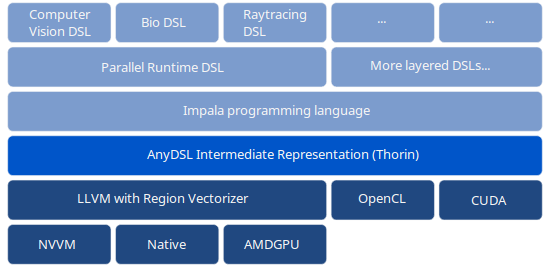
\includegraphics[width=13cm]{anydsl_architecture.png}
\caption{AnyDSL architecture, the DSL code is written using the Impala front-end language, then compiled into the Thorin representation to be finally compiled to the specified backend.}
\label{fig:anydsl_architecture}
\end{figure}

For our work, we compiled our input program with the Impala compiler emitting LLVM IR code, when we link the sources with the GPU backend, the compiler generates a C/C++ CUDA source containing the kernels specificiations, as well as the file containing the LLVM IR of the code to be executed in the host. Our work focus on changing the code generation of the C/C++ CUDA source.

After generating the sources mentioned above, we use the Clang compiler to generate our final executable file by compiling the LLVM IR of the host program and compiling and linking extra C/C++ code into LLVM IR, these extra codes have the OpenCV \cite{opencv} functions to read and write images from PNG files.

Finally, the executable generated may be executed and it will perform Just-In-Time (JIT) compilation of the CUDA C/C++ code during its execution.

\section{Gaussian blur}
The Gaussian blur operator is used for blurring the image removing its noise. To transform the image using the Gaussian operator it's necessary to convolve each pixel of the image with the Gaussian function defined as follows:

\begin{equation*}
    G(x,y) = \frac{1}{\sqrt{2\pi\sigma^2}}e^{-\frac{x^2 + y^2}{2\sigma^2}}
\end{equation*}

An example of kernel that may be used to apply the Gaussian smooth is shown below:

\begin{equation*}
K = \frac{1}{159}
\begin{bmatrix}
2 & 4 & 5 & 4 & 2\\
4 & 9 & 12 & 9 & 4\\
5 & 12 & 15 & 12 & 5\\
2 & 4 & 5 & 4 & 2\\
4 & 9 & 12 & 9 & 4\\
\end{bmatrix}
\end{equation*}

The Figure \ref{fig:gaussian_example} shows an example of the Gaussian blur filter. It's also noticeable that our version generates output images in grayscale for simplicity purposes.

\begin{figure*}[t!]
    \centering
    \begin{subfigure}
        \centering
        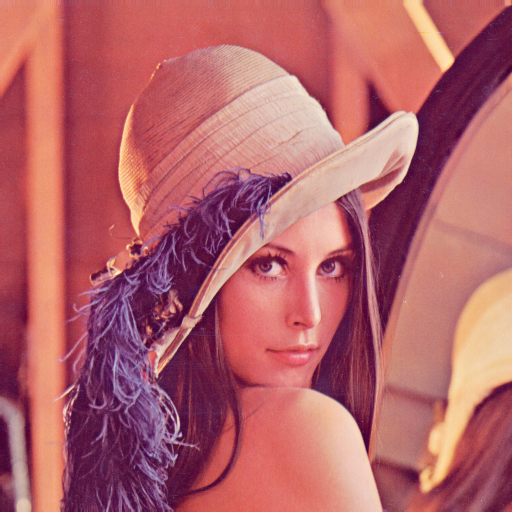
\includegraphics[height=1.2in]{lenna.png}
    \end{subfigure}%
    ~ 
    \begin{subfigure}
        \centering
        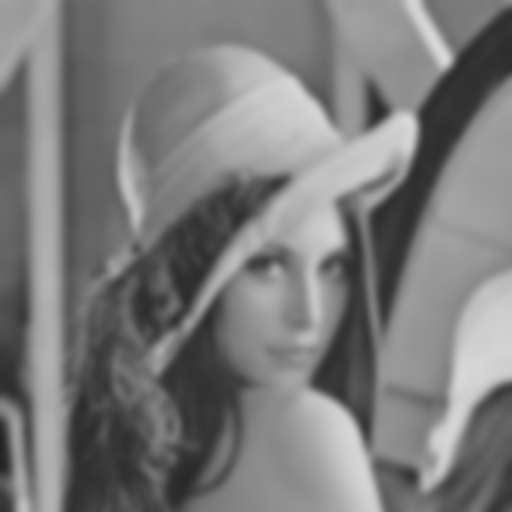
\includegraphics[height=1.2in]{lenna_gaussianblur.jpg}
    \end{subfigure}
    \caption{Gaussian filter example, left figure shows the original image and right figure shows the result after the Gaussian blur.}

\label{fig:gaussian_example}
\end{figure*}

\pagebreak

The code below shows our implementation of the Gaussian blur, in the \textbf{gaussian\_blur} function, the filter coeffiecients are calculated for both unidimensional and bidimensional filters and then the functions for applying the convolution (for separable and block filters) are called with the generated filter.

\begin{minted}{rust}
/* Gaussian filter */
fn gaussian_blur(input_image : image, output_image : image, use_tiled : bool) -> () {
  /* Generates the separable or non-separable Gaussian kernel based on the
     OpenCV source code */
  let filter_size = 7;
  let filter_Nx1 = filter_7x1;
  let filter_NxN = filter_7x7;

  /* Allocate CPU memory for the mask buffers (block, row and column) */
  let bmask_xy = alloc_cpu(filter_size * filter_size * sizeof[f64]());
  let bmask_x = alloc_cpu(filter_size * sizeof[f64]());
  let bmask_y = alloc_cpu(filter_size * sizeof[f64]());

  /* Pointers to the buffers in f64 data type */
  let mask_xy = bmask_xy.data as &mut[f64];
  let mask_x = bmask_x.data as &mut[f64];
  let mask_y = bmask_y.data as &mut[f64];

  /* The next steps generate the gaussian filter for both block as well as horizontal
     and vertical kernels */
  let mut sum_x = 0.0;
  let mut sum_y = 0.0;
  let anchor = 2.0;
  let pi = 3.14159;
  let sigma = 1.1;
  let prod = 1.0 / (2.0 * pi * sigma * sigma);
  let denom = 2.0 * sigma * sigma;

  for i in range(0, filter_size) {
    let x = (i as f64) - anchor;

    for j in range(0, filter_size) {
      let y = (j as f64) - anchor;

      mask_xy(j * filter_size + i) = prod * exp(-((x * x + y * y) / denom));
    }

    mask_x(i) = exp(-((x * x) / denom));
    mask_y(i) = exp(-((x * x) / denom));
    sum_x += mask_x(i);
    sum_y += mask_y(i);
  }

  sum_x = 1.0 / sum_x;
  sum_y = 1.0 / sum_y;

  for i in range(0, filter_size) {
    mask_x(i) *= sum_x;
    mask_y(i) *= sum_y;
  }

  /* Time calculation variables */
  let mut start_time : f64;
  let mut elapsed_time : f64;

  /* Applies the separable kernel in rows and columns */
  if use_tiled {
    let column_filter = filter_Nx1(bmask_x, false);
    let row_filter = filter_Nx1(bmask_y, true);

    start_time = impala_time();
    apply_separable_convolution(input_image, output_image, column_filter, row_filter);
    elapsed_time = impala_time() - start_time;

    release_filter(column_filter);
    release_filter(row_filter);
  /* Applies the not separable kernel in blocks */
  } else {
    let block_filter = filter_NxN(bmask_xy);

    start_time = impala_time();
    apply_block_convolution(input_image, output_image, block_filter);
    elapsed_time = impala_time() - start_time;

    release_filter(block_filter);
  }

  print_string("Time elapsed: ");
  print_f64(elapsed_time);
  print_string("s\n");

  /* Release memory for the mask buffers */
  release(bmask_xy);
  release(bmask_x);
  release(bmask_y);
}
\end{minted}

\pagebreak

The code below shows the implementation of the \textbf{apply\_separable\_convolution} function for applying the separable unidimensional Gaussian filters. We limit our experiments to the separable kernel application so we only show it in this report.

\begin{minted}{rust}
/* Apply 2D filter convolution with separable kernels (tiling) */
fn apply_separable_convolution(input_image : image, output_image : image, h_mask : filter, v_mask : filter) -> () {
  /* Horizontal anchor based in the horizontal mask size */
  let h_anchor = h_mask.width / 2;
  /* Vertical anchor based in the vertical mask size */
  let v_anchor = v_mask.height / 2;

  /* Allocate temporary data in the target device for holding the row convolution result */
  let tmp_image = create_temporary_image(input_image.width, input_image.height);

  /* Applies the filter in columns */
  for x, y, input, filt in @iterate_stencil(input_image, h_mask) {
    /* Sum is 0.0 by default */
    let mut sum = 0.0;

    /* Check image boundaries to avoid invalid memory region access */
    if x >= h_anchor && x < input_image.width - h_anchor {
      /* Go through the horizontal mask coefficients using the specified anchor */
      for i in range(-h_anchor, h_anchor + 1) {
        /* Increase the current coefficient and input product in the summation */
        sum += get_1d_filter_coeff(filt, i + h_anchor) * get_pixel(input, x + i, y);
      }

      /* Write the summation result in the temporary buffer */
      set_pixel(tmp_image, x, y, sum);
    /* If this is an invalid region, just copy the input pixel value to the temporary buffer */
    } else {
      /* Use original input value */
      set_pixel(tmp_image, x, y, get_pixel(input, x, y));
    }
  }

  /* Applies the filter in rows */
  for x, y, input, filt in @iterate_stencil(tmp_image, v_mask) {
    /* Sum is 0.0 by default */
    let mut sum = 0.0;

    /* Check image boundaries to avoid invalid memory region access */
    if y >= v_anchor && y < input_image.height - v_anchor {
      /* Go through the vertical mask coefficients using the specified anchor */
      for i in range(-v_anchor, v_anchor + 1) {
        /* Increase the current coefficient and input product in the summation */
        sum += get_1d_filter_coeff(filt, i + v_anchor) * get_pixel(input, x, y + i);
      }

      /* Write the summation result in the output buffer */
      set_pixel(output_image, x, y, sum);
    /* If this is an invalid region, just copy the temporary pixel value to the output buffer */
    } else {
      /* Use original input value */
      set_pixel(output_image, x, y, get_pixel(input, x, y));
    }
  }

  /* Release memory for temporary buffer */
  release_image(tmp_image);
}
\end{minted}

In the first part, the horizontal filter is applied in the image and its result is stored in a temporary image. After, the vertical filter is applied in the temporary image and its result is stored in the output image. The \textbf{iterate\_stencil}, \textbf{get\_1d\_filter\_coeff}, \textbf{get\_pixel} and \textbf{set\_pixel} functions are used to abstract the architecture and they are implemented in the device-specific Impala files that must be linked during the Gaussian blur compilation.

The following code show these functions implementation for the CUDA GPU devices:

\begin{minted}{rust}
/* Sets image pixel at (x, y) coordinates */
fn set_pixel(img : image, x : i32, y : i32, value : f64) -> () {
  bitcast[&mut[1][f64]](img.device_data.data)(y * img.width + x) = value
}

/* Gets image pixel at (x, y) coordinates */
fn get_pixel(img : image, x : i32, y : i32) -> f64 {
  bitcast[&[1][f64]](img.device_data.data)(y * img.width + x)
}

/* Gets 1D filter coefficient at i index */
fn get_1d_filter_coeff(filt : filter, i : i32) -> f64 {
  bitcast[&[1][f64]](filt.buffer.data)(i)
}
...
/* Iterates over an image in GPU based on a stencil */
fn iterate_stencil(input_image : image, stencil : filter, body: fn(i32, i32, image, filter) -> ()) -> () {
  /* Use first CUDA accelerator */
  let accelerator = cuda_accelerator(0);
  /* CUDA kernel grid configuration */
  let grid = get_grid_config(input_image);
  /* CUDA kernel block configuration */
  let block = get_block_config();

  /* Execute the following code in the GPU */
  with accelerator.exec(grid, block) @{
    /* Image x coordinate in the grid */
    let gid_x = accelerator.bidx() * accelerator.bdimx() + accelerator.tidx();
    /* Image y coordinate in the grid */
    let gid_y = accelerator.bidy() * accelerator.bdimy() + accelerator.tidy();

    /* Check for image boundaries to avoid invalid memory region access */
    if gid_x < input_image.width && gid_y < input_image.height {
      /* Call the body function with the obtained indexes */
      body(gid_x, gid_y, input_image, stencil);
    }
  }
}
\end{minted}

Our optimizations work in the kernel generated by the \textbf{accelerator.exec(grid, block)} function that triggers the Thorin code generation for CUDA backend. We emit the copy of the \textbf{input\_image} to the shared memory and replace the accesses to the \textbf{input\_image} for accesses to the shared memory, the procedure is analogous for the \textbf{stencil}.

\section{Methodology}
Thorin is a CPS graph based higher-order intermediate representation, this means that its code generator will iterate over the graph generating its continuations, parameters and primops. For each vertex in the graph, Thorin must generate a unique name to avoid conflicts, our idea is to trace some of these vertex by the name to identify the filters and images in the kernel parameters (we also use the names of the structures in our experimental DSL in Impala for this).

After knowing the images and filters in the kernel, we trace their buffers so we know if they are read-only buffers or if at some point in the code they will be written. In the second case, we ignore them as we don't want to store writable buffers in the shared memory.

In the first step of the code generation we define a macro with the filter size used, then at each kernel declaration, we get the kernel block dimensions and emit the shared memory buffer declarations for both image and filter.

Before the next code generation we go through the Thorin graph to perform an initial analysis, going through the kernel primops to check the parameters behavior, if an extraction, a bitcast or a LEA operation is performed on a buffer that comes from an image or filter of the kernel, we keep saving the sources. This step are used for the read-only buffers tracing technique mentioned above. When we find a load operation in one of our targets, we insert them in the shared memory candidates list if they weren't blacklisted yet. A target is blacklisted when a store operation is performed in it (we don't want to store writable kernel buffers in the shared memory).

After the analysis, we go generating the code and for each bitcasting operation with the targets we emit the shared memory copy of the original buffer in the slow global memory to the faster memory by splitting the buffer in blocks of the kernel block dimension. Then we iterate over each buffer blocks with each thread transferring one element (per iteration) from the global memory to the faster memory. Finally, for each LEA operation with a target, we change the target reference to the shared memory with the offsets (x and y axis) included in the indexes.

This methodology of listing the candidates, tracing their path to know which ones are read-only and then during the code generation generating the copy and replacing the accesses for the candidates is used on this work to perform the shared memory code generation. The next section shows the code changed in the Thorin code generator for a practical guide through this work's idea.

\section{Changes in the code generator}

We use lists (C++ \textbf{std::list}) to perform the analysis, the \textbf{kernel\_images} and \textbf{kernel\_filters} lists will contain all the image and filter references from the kernel, respectively. The \textbf{image\_pointers} and \textbf{filter\_pointers} lists will have all the direct and indirect references to the image and filter buffers, respectively (doesn't matter which type these references have). The \textbf{shm\_buffers} list will contain all the selected buffers that must go to the shared memory and the \textbf{shm\_blacklist} will contain all the blacklisted buffers. The \textbf{std::map} object \textbf{conv\_map} contains the association between \textbf{image\_pointers} and \textbf{filter\_pointers} objects and their \textbf{shm\_buffers} object.

\subsection{Data structures}

\begin{minted}{cpp}
static std::list<std::string> shm_buffers;
static std::list<std::string> shm_blacklist;
static std::list<std::string> kernel_images;
static std::list<std::string> kernel_filters;
static std::list<std::string> image_pointers;
static std::list<std::string> filter_pointers;
static std::map<std::string, std::string> conv_map;
\end{minted}

The following code shows the functions that emits the copy from the global memory to the shared memory for an image giving the shared memory name \textbf{shm\_name} and the source buffer pointer \textbf{src\_buffer} name to be copied. The \textbf{adjusted\_(shm\_name)} definition in the end of the code is used for further accesses into the shared memory. \textbf{FILTER\_SIZE} holds the filter size.

\pagebreak

\subsection{Image shared memory functions}

\begin{minted}{cpp}
std::ostream& CCodeGen::emit_shm_image_copy(const std::string shm_name, const std::string src_buffer) {
  int extend_width = FILTER_SIZE / 2;
  int extend_height = FILTER_SIZE / 2;

  std::string idxx_string = "gidx - " + std::to_string(extend_width) + " + i";
  std::string idxy_string = "gidy - " + std::to_string(extend_height) + " + j";

  func_impl_ << endl;

  func_impl_ << "#line 100 \"shared_memory_image_copy\"" << endl;
  func_impl_ << "int gidx = blockIdx.x * blockDim.x + threadIdx.x;" << endl;
  func_impl_ << "int gidy = blockIdx.y * blockDim.y + threadIdx.y;" << endl;

  func_impl_ << "for(int i = 0; threadIdx.x + i < blockDim.x + " << extend_width * 2 << "; i += blockDim.x) {" << up << endl;
  func_impl_ << "int idxx = " << idxx_string << ";" << endl;

  func_impl_ << "for(int j = 0; threadIdx.y + j < blockDim.y + " << extend_height * 2 << "; j += blockDim.y) {" << up << endl;
  func_impl_ << "int idxy = " << idxy_string << ";" << endl;

  func_impl_ << "if(idxx < image_width_reg && idxy < image_height_reg) {" << up << endl;

  func_impl_ << shm_name << "[(threadIdx.y + j) * " << shm_width << " + threadIdx.x + i] = " << \
                src_buffer << "[idxy * image_width_reg + idxx];" << down << endl;

  func_impl_ << "}" << down << endl;
  func_impl_ << "}" << down << endl;
  func_impl_ << "}" << endl;

  func_impl_ << endl << "__syncthreads();" << endl;

  func_impl_ << endl << "double *adjusted_" << shm_name << " = &" << shm_name << \
                        "[(" << extend_height << " - blockIdx.y * blockDim.y) * " << shm_width << \
                        " + " << extend_width << " - blockIdx.x * blockDim.x];" << endl;

  return func_impl_;
}
\end{minted}

The following code shows the function that emits the shared memory access for an image giving its name in \textbf{shm\_name} and its \textbf{x} and \textbf{y} positions.

\begin{minted}{cpp}
std::ostream& CCodeGen::emit_shm_image_access(const std::string shm_name, std::string x, std::string y) {
  func_impl_ << "&" << "adjusted_" << shm_name << "[(" << y  << ") * " << shm_width << " + (" << x << ")]";

  return func_impl_;
}
\end{minted}

\subsection{Filter shared memory functions}

The following code shows the functions that emits the copy from the global memory to the shared memory for a filter giving the shared memory name \textbf{shm\_name} and the source buffer pointer \textbf{src\_buffer} name to be copied. The \textbf{SEP\_FILTER} macro defines if it's an unidimensional separable filter or it's a bidimensional block filter. \textbf{FILTER\_SIZE} contains the filter size.

\pagebreak

\begin{minted}{cpp}
std::ostream& CCodeGen::emit_shm_filter_copy(const std::string shm_name, const std::string src_buffer) {
  std::string idx_string;

  func_impl_ << endl;

  func_impl_ << "#line 200 \"shared_memory_filter_copy\"" << endl;

#ifdef SEP_FILTER
  idx_string = "i";

  func_impl_ << "for(int i = 0; i < " << FILTER_SIZE << "; i++) {" << up << endl;
  func_impl_ << shm_name << "[" << idx_string << "] = " << src_buffer << "[" << idx_string << "];" << down << endl;

  func_impl_ << "}" << endl;
#else
  idx_string = "(threadIdx.y + j) * " + std::to_string(FILTER_SIZE) + " + threadIdx.x + i";

  func_impl_ << "for(int i = 0; i < " << FILTER_SIZE << "; i += blockDim.x) {" << up << endl;
  func_impl_ << "for(int j = 0; j < " << FILTER_SIZE << "; j += blockDim.y) {" << up << endl;
  func_impl_ << "if(threadIdx.x + i < " << FILTER_SIZE << " && " << endl << \
                "   threadIdx.y + j < " << FILTER_SIZE << ") {" << up << endl;

  func_impl_ << shm_name << "[" << idx_string << "] = \\" << endl << \
                "  " << src_buffer << "[" << idx_string << "];" << down << endl;

  func_impl_ << "}" << down << endl;
  func_impl_ << "}" << down << endl;
  func_impl_ << "}" << endl;
#endif

  func_impl_ << endl << "__syncthreads();" << endl;

  return func_impl_;
}
\end{minted}

The following code shows the function that emits the shared memory access for a filter giving its name in \textbf{shm\_name} and the index \textbf{index} to be accessed.

\begin{minted}{cpp}
std::ostream& CCodeGen::emit_shm_filter_access(const std::string shm_name, std::string index) {
  func_impl_ << "&" << shm_name << "[" << index << "]";

  return func_impl_;
}
\end{minted}

\subsection{Kernel image and filter identification}

The following code will use our experimental DSL structure names \textbf{image} and \textbf{filter} to select the kernel parameters that are images or filters. We also include the AnyDSL structure \textbf{Buffer} to be considered as images because of the second kernel in the separable convolution that receives the image as \textbf{Buffer} instead of \textbf{image}.

\begin{minted}{cpp}
std::stringstream type_stream;

type_stream << param->type();

if(type_stream.str().compare("filter") == 0 && !list_contains(kernel_filters, param->unique_name())) {
  kernel_filters.push_back(param->unique_name());
}

if(type_stream.str().compare("image") == 0 && !list_contains(kernel_images, param->unique_name())) {
  image_width_name = param->unique_name() + ".e2";
  image_height_name = param->unique_name() + ".e3";
  kernel_images.push_back(param->unique_name());
}

if(type_stream.str().compare("Buffer") == 0 && !list_contains(kernel_images, param->unique_name())) {
  kernel_images.push_back(param->unique_name());
}
\end{minted}

The \textbf{e2} and \textbf{e3} elements in the image strucuture holds the image width and height, respectively.

\subsection{Shared memory declarations}

The following code emits the shared memory declaration in the kernel using the \textbf{FILTER\_SIZE} macro.

\begin{minted}{cpp}
if(bdimx != 0 && bdimy != 0 && bdimz != 0) {
  shm_width = bdimx + (FILTER_SIZE / 2) * 2;
  func_impl_ << endl << "__shared__ double ds_img[" << (shm_width * (bdimy + (FILTER_SIZE / 2) * 2)) << "];";

  #ifdef SEP_FILTER
    func_impl_ << endl << "__shared__ double ds_filter[" << FILTER_SIZE << "];";
  #else
    func_impl_ << endl << "__shared__ double ds_filter[" << (FILTER_SIZE * FILTER_SIZE) << "];";
  #endif
}
\end{minted}

\subsection{Read-only buffers tracing}

The following code is executed before the code generation, it perform our analysis of possible candidates to be optimized using the shared memory.

\begin{minted}{cpp}
for(const auto& block : schedule) {
  auto continuation = block.continuation();
  if(continuation->empty()) {
    continue;
  }

  assert(continuation == scope.entry() || continuation->is_basicblock());

  for(auto primop : block) {
    auto primop_name = var_name(primop);

    if(auto aggop = primop->isa<AggOp>()) {
      if(aggop->isa<Extract>()) {
        if(list_contains(kernel_images, aggop->agg()->unique_name())) {
          if(aggop->type()->isa<StructType>() && !list_contains(kernel_images, primop_name)) {
            kernel_images.push_back(primop_name);
          } else if(aggop->type()->isa<PtrType>() && !list_contains(image_pointers, primop_name)) {
            image_pointers.push_back(primop_name);
          }
        }

        if(list_contains(kernel_filters, aggop->agg()->unique_name())) {
          if(aggop->type()->isa<StructType>() && !list_contains(kernel_filters, primop_name)) {
            kernel_filters.push_back(primop_name);
          } else if(aggop->type()->isa<PtrType>() && !list_contains(filter_pointers, primop_name)) {
            filter_pointers.push_back(primop_name);
          }
        }
      }
    } else if(auto conv = primop->isa<ConvOp>()) {
      if(conv->isa<Bitcast>()) {
        if(list_contains(image_pointers, conv->from()->unique_name())) {
          image_pointers.push_back(primop_name);
        }

        if(list_contains(filter_pointers, conv->from()->unique_name())) {
          filter_pointers.push_back(primop_name);
        }
      }
    } else if(auto lea = primop->isa<LEA>()) {
      if(list_contains(image_pointers, lea->ptr()->unique_name())) {
        conv_map.insert(std::pair<std::string, std::string>(lea->ptr()->unique_name(), primop_name));
        image_pointers.push_back(primop_name);
      }

      if(list_contains(filter_pointers, lea->ptr()->unique_name())) {
        conv_map.insert(std::pair<std::string, std::string>(lea->ptr()->unique_name(), primop_name));
        filter_pointers.push_back(primop_name);
      }
    } else if(auto load = primop->isa<Load>()) {
      auto ptr_name = load->ptr()->unique_name();
      auto blacklisted = list_contains(shm_blacklist, ptr_name);

      if(!blacklisted && (list_contains(image_pointers, ptr_name) || list_contains(filter_pointers, ptr_name))) {
        shm_buffers.push_back(ptr_name);
      }
    } else if(auto store = primop->isa<Store>()) {
      auto ptr_name = store->ptr()->unique_name();

      if(list_contains(shm_buffers, ptr_name)) {
        shm_buffers.remove(ptr_name);
      }

      shm_blacklist.push_back(ptr_name);
    }
  }
}
\end{minted}

\subsection{Dimension registers}

The next code generation is used to generate the registers \textbf{image\_width\_reg} and \textbf{image\_height\_reg} with the image dimensions. This is used so we have a known name for these values and also to avoid structure element access each time we use them.

\begin{minted}{cpp}
func_impl_ << endl;
func_impl_ << "int image_width_reg = " << image_width_name << ";" << endl;
func_impl_ << "int image_height_reg = " << image_height_name << ";" << endl;
\end{minted}

\subsection{Shared memory copy generation}

The code below shows the shared memory copy code generation after the bitcast operation (irrelevant parts of the code were omitted for legibility purposes).

\begin{minted}{cpp}
if (conv->isa<Bitcast>()) {
    ...

    if(list_contains(image_pointers, def_name)) {
      std::map<std::string, std::string>::iterator i;

      if((i = conv_map.find(def_name)) != conv_map.end()) {
        if(list_contains(shm_buffers, i->second)) {
          emit_shm_image_copy("ds_img", def_name);
        }
      }
    }

    if(list_contains(filter_pointers, def_name)) {
      std::map<std::string, std::string>::iterator i;

      if((i = conv_map.find(def_name)) != conv_map.end()) {
        if(list_contains(shm_buffers, i->second)) {
          emit_shm_filter_copy("ds_filter", def_name);
        }
      }
    }
}
\end{minted}

\subsection{Shared memory access generation}

Finally, the next code emits the shared memory access when necessary in the LEA operations (irrelevant parts of the code were omitted for legibility purposes).

\begin{minted}{cpp}
if (auto lea = def->isa<LEA>()) {
    if (is_texture_type(lea->type())) { // handle texture fetches
      ...
    } else {
        if (lea->ptr_pointee()->isa<TupleType>() || lea->ptr_pointee()->isa<StructType>()) {
          ...
        } else if (lea->ptr_pointee()->isa<DefiniteArrayType>()) {
          ...
        } else {
            if(list_contains(shm_buffers, def_name)) {
              func_impl_ << "#line 100 \"shared_memory_access\"" << endl;
            }

            emit_addr_space(func_impl_, lea->ptr()->type());
            emit_type(func_impl_, lea->type()) << " " << def_name << ";" << endl;
            func_impl_ << def_name << " = ";

            if(list_contains(shm_buffers, def_name)) {
                std::map<std::string, std::string>::iterator i;
                auto is_filter = list_contains(filter_pointers, def_name);

                if(!is_filter) {
                  emit_shm_image_access(
                    "ds_img",
                    lea->index()->unique_name() + " % image_width_reg",
                    lea->index()->unique_name() + " / image_width_reg"
                  );
                } else {
                  emit_shm_filter_access("ds_filter", lea->index()->unique_name());
                }

                func_impl_ << ";"; 
            } else { 
                emit(lea->ptr()) << " + ";
                emit(lea->index()) << ";"; 
            }
        }
    }

    ...
}
\end{minted}

\section{Experimental Results}

To perform the experiments and validate our generated code version performance, we use the Berkeley Segmentation Dataset \cite{dataset} available at \cite{dataseturl}, which contains 100 images with 321x481 and 481x321 dimensions. As these dimensions are too small for performance comparison, we use the same procedure as \cite{luislourenco} to generate the variations with higher dimensions.

Considering the original dataset images as the B1 dataset, we generate the B2 dataset with the doubled dimensions by repeating the original images vertically, horizontally and diagonally. So, we repeat the same procedure on B2 to generate the B3 dataset, and the same on B3 to generate the B4 dataset. After all we have the following dimensions: 321x481 and 481x321 for B1 dataset, 642x962 and 962x642 for B2 dataset, 1284x1924 and 1924x1284 for B3 dataset and 2568x3848 and 3848x2568 for B4 dataset, all of them containing 100 images each.

The performance tests were performed using a GeForce GT 710 graphic board with 192 CUDA cores, 954MHz base clock, 2GB of memory with 1.8 Gbps of speed and a 64-bit DDR3 memory interface. We execute three different versions for all the images on each dataset and considered the summation of the times as the final result for our tests. The mentioned versions are named \textbf{no\_shm} for the original AnyDSL version that doesn't use shared memory, \textbf{shm\_filteronly} version that only uses shared memory for filter and \textbf{shm\_both} version that uses shared memory for both image and filter.

The Figure \ref{fig:results} shows the result in seconds for each dataset and the Table \ref{table:speedups} shows the speedups for \textbf{shm\_filteronly} and \textbf{shm\_both} versions.

\begin{figure}[!htb]
\centering
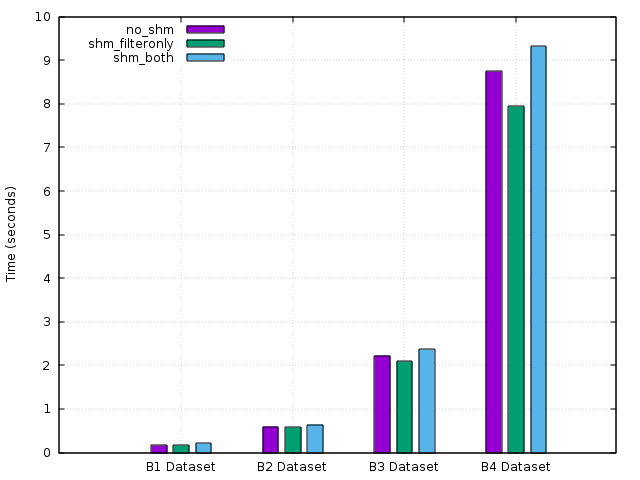
\includegraphics[width=13cm]{results.png}
\caption{Results for B1, B2, B3 and B4 datasets.}
\label{fig:results}
\end{figure}

\begin{table}
\centering
\begin{tabular}{ | c | c | c | c | c | }
  \hline
  & B1 & B2 & B3 & B4 \\
  \hline
  \textbf{shm\_filteronly} & 1.01144963524 & 1.01751663664 & 1.06079745639 & 1.10045501174 \\
  \hline
  \textbf{shm\_both} & 0.80856073526 & 0.92615324824 & 0.93869369236 & 0.93835056282 \\
  \hline
\end{tabular}
\caption{Speedups for \textbf{shm\_filteronly} and \textbf{shm\_both} versions}
\label{table:speedups}
\end{table}

The results shows that our version that only uses shared memory for filter is better than the original, while the version with both filter and image performed worse than the others. According to our analysis, this happened because of the emitted accesses for the image using the module and division functions with the image width to remap the original image index to the shared memory index.

To achieve a better result for the \textbf{shm\_both} version, a more sophisticated analysis would be required to identify the loops that originally traverse the global memory and change their range so we can directly access the shared memory without previous calculation of the index. We performed basic tests by generating constant values in the shared memory accesses for the image that got better performance results than the original version without shared memory, but these aren't considered valid results for this work as they change the output result, instead they may present an evidence that the performance problem of the \textbf{shm\_both} is actually in the shared memory index access.

\section{Future Work}
Future work may include a better way to remap the accesses from the global memory to the shared memory (by identifying the loops in the code and changing their range), as well as perform other kinds of optimizations during the code generation.

Another interesting work would be to perform the same optimizations for other GPU frameworks like OpenCL for example, then an analysis of performance using the modified version for a different architecture could be achieved.

Also, it's interesting to perform the experiments using a GPU with more Streaming Multiprocessors (SMs) since the used GPU only has one, this is import for testing and compare the scalability of the optimized program in relation to the base.

\section{Conclusion}
The work in this report changes the Thorin generated code for the CUDA backends to include shared memory usage in the final version. We show better results for performance on inserting the filter into the shared memory (about 10\% of speedup for the tested cases) and identified problems on remapping the image accesses to the shared memory (in relation to performance).

\begin{thebibliography}{4}

\bibitem{anydsl}
  https://anydsl.github.io/

\bibitem{opencv}
  https://opencv.org/

\bibitem{dataseturl}
   Arbelaez, P. and Fowlkes, C. and Martin, D.,
   \textit{The Berkeley Segmentation Dataset and Benchmark 2007},
   http://www.eecs.berkeley.edu/Research/Projects/CS/vision/bsds/,
   2007,
   Acessado em 04/05/2017.

\bibitem{dataset}
  D. Martin and C. Fowlkes and D. Tal and J. Malik,
  \textit{A Database of Human Segmented Natural Images and its 
           Application to Evaluating Segmentation Algorithms and 
           Measuring Ecological Statistics},
  Proc. 8th Int'l Conf. Computer Vision,
  2001,
  July,
  2,
  416--423.

\bibitem{luislourenco}
   Luis Henrique Alves Lourenço,
   \textit{Paralelização do Detector de Bordas Canny para a biblioteca ITK utilizando CUDA},
   Pós-Graduação em Informática - Universidade Federal do Paraná, 
   2011.

\end{thebibliography}

\end{document}

